\chapter{Thực nghiệm}
Với mục tiêu tìm hiểu và giải quyết bài toán phân loại thực khuẩn với dữ liệu đầu vào là contig, nhóm sinh viên thực hiện các thử nghiệm và đánh giá tương tự với nhóm tác giả DeePhage. Chương này trình bày phương pháp xây dựng bộ dữ liệu, các chỉ số đánh giá, kịch bản và kết quả thực nghiệm.

\section{ Xây dựng bộ dữ liệu}
\subsection{ Xử lý nhãn }
Sau khi tìm hiểu các bài báo, nhóm sinh viên thực hiện xây dựng bộ dữ liệu mới dựa trên 2 bộ dữ liệu được sử dụng trong bài báo DeepPL và DeePhage. Nhãn $y$ của bản ghi $X$ được nhóm sinh viên xử lý như sau:
\begin{enumerate}
    \item Nếu $X \in DeePhage \Rightarrow y = y_{DeePhage}$ 
    \item Nếu $X \in DeepPL \Rightarrow y = y_{DeepPL}$
    \item Nếu $X \in DeePhage \cap DeepPL \Rightarrow y = y_{DeePhage}$
\end{enumerate}

\subsection{ Chia tập dữ liệu}
Sau khi thực hiện gộp 2 bộ dữ liệu DeePhage và DeepPL, nhóm sinh viên xử lý dữ liệu theo 4 bước sau:
\begin{enumerate}
    \item Chia bộ dữ liệu thành 2 tập: huấn luyện và kiểm thử.
    \item Sử dụng kỹ thuật cửa sổ trượt, tạo các đoạn contig từ bộ gen đầy đủ với 4 nhóm độ dài khác nhau. Khi thực hiện tạo ra các contig, nhóm đã cài đặt đoạn cửa sổ sau sẽ có sự trùng lặp 30\% so với đoạn cửa số trước và phân bố độ dài các contig trong 1 nhóm tuân theo phân bố chuẩn.
    \begin{itemize}
        \item A: 100 bp - 400 bp
        \item B: 400 bp - 800 bp
        \item C: 800 bp - 1200 bp
        \item D: 1200 bp - 1800 bp
    \end{itemize}
    \item Thực hiện véc-tơ hóa dữ liệu. Tại bước này, nhóm sinh viên sử dụng 2 phương pháp véc-tơ hóa dữ liệu: One-hot và Word2Vec để phù hợp với 2 kịch bản thực nghiệm được trình bày tại phần \ref{ kịch bản thực nghiệm}
    \begin{itemize}
        \item Sử dụng One-hot đối với phương pháp DeePhage.
        \item Sử dụng Word2Vec với k-mer=6.
    \end{itemize}
    \item Áp dụng Random Undersampling để cân bằng phân phối nhãn của bộ dữ liệu.
\end{enumerate}

\section{Kịch bản thực nghiệm}\label{ kịch bản thực nghiệm}
Để tiến hành các thực nghiệm, nhóm sinh viên chọn 2 mô hình là DeePhage và XGBoost. Nhận thấy DeePhage là công cụ toàn diện hơn so với nhóm công cụ dựa trên Bert do DeePhage có thể thực hiện phân loại trên nhiều nhóm contig có đội dài linh hoạt, trong khi nhóm công cụ dựa trên Bert chỉ được đánh giá trên bộ dữ liệu có độ dài đầu vào nhỏ hơn bằng 512 bp, nhóm sinh viên quyết định chọn DeePhage là công cụ tiêu chuẩn trong các thực nghiệm. Ngoài ra, do cần 1 mô hình đủ mạnh để có thể có hiệu suất phân loại tốt cũng như nhanh trong quá trình huấn luyện, nhóm quyết định chọn XGBoost là mô hình được sử dụng để trực tiếp so sánh với DeePhage.

Nhóm sinh viên thực hiện 2 kịch bản:
\begin{enumerate}
    \item Kiểm tra hiệu suất phân loại của DeePhage trên bộ dữ liệu xây dựng.
    \item Kiểm tra hiệu suất phân loại của XGBoost trên bộ dữ liệu xây dựng. (Có nên giải thích tại sao chọn XGBoost không?)
    % \item Thực hiện so sánh hiệu suất phân loại của DeePhage và XGBoost.
\end{enumerate}

% Với kịch bản 1, nhóm sinh viên thực hiện những công việc sau
% 1. Dưa trên code của tác giả, chuyển code về pytorch
% 2. Sử dụng One-hot để véc-tơ hóa dữ liệu
% 3. Thử nghiệm mô hình với bộ dữ liệu xây dựng.

% Với kịch bản 2, nhóm sinh viên thực hiện:
% 1. Cài đặt thực nghiệm với XGBoost 
% 2. Thử nghiệm mô hình với bộ dữ liệu được véc-tơ hóa thông qua Word2Vec.

\section{Các chỉ số đánh giá}
Để đánh giá 1 cách toàn diện hiệu suất phân loại của mô hình chứ không chỉ tập trung vào nhãn 1, nhóm sinh viên sử dụng các chỉ số sau:
\begin{itemize}
    \item Accuracy: sử dụng để do lường hiệu suất phân loại chung của mô hình trên 2 nhãn.
    \item Sensitivity: sử dụng để đo lường dộ phủ của mô hình trên nhãn 1.
    \item Specificity: sử dụng để đo lường độ phủ của mô hình trên nhãn 0.
\end{itemize}
Ngoài những chỉ số trên, các chỉ số Precision, F1, ROC\_AUC cũng được sử dụng trong kịch bản 2.

\section{Kết quả}
\subsection{Hiệu suất phân loại của DeePhage trên bộ dữ liệu xây dựng}

\begin{figure}[H]
    \centering
    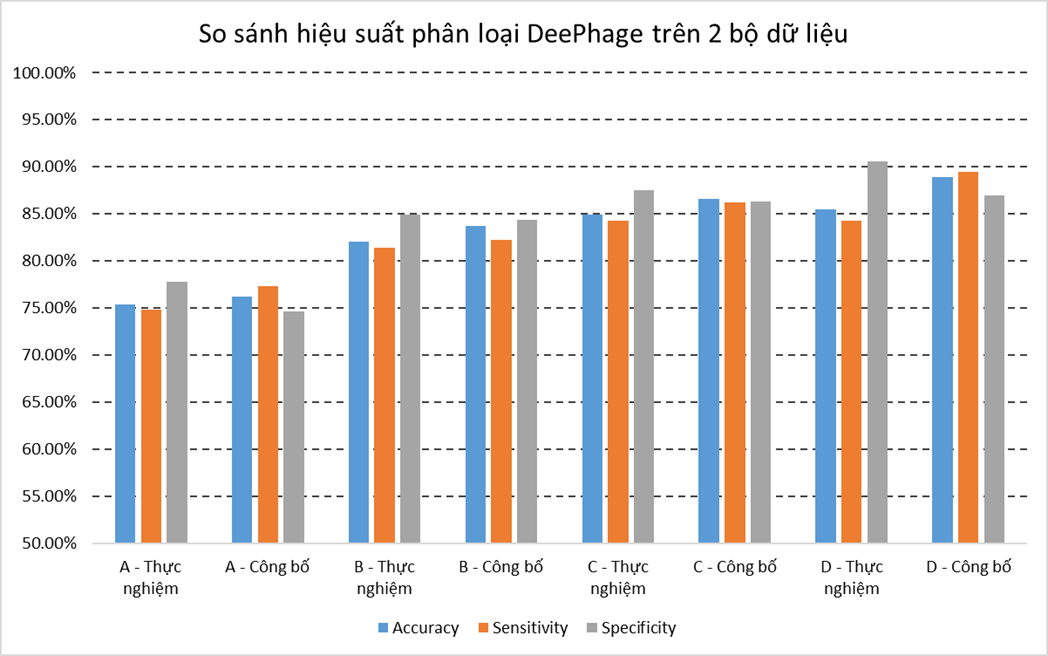
\includegraphics[width=1\linewidth]{figures/result_deephage_exp_vs_paper.png}
    \caption{So sánh hiệu suất phân loại của mô hình DeePhage trên 2 bộ dữ liệu xây dựng và công bố.}
    \label{fig:result_1}
\end{figure}

Từ Hình \ref{fig:result_1}, ta có thể thấy mức độ chênh lệch giữa kết quả của DeePhage trên bộ dữ liệu được nhóm sinh viên xây dựng và kết quả được công bố có độ chênh lệch ở mức hợp lý, không quá 5\%.

\subsection{Hiệu xuất phân loại của XGBoost trên bộ dữ liệu xây dựng}

\begin{figure}[H]
    \centering
    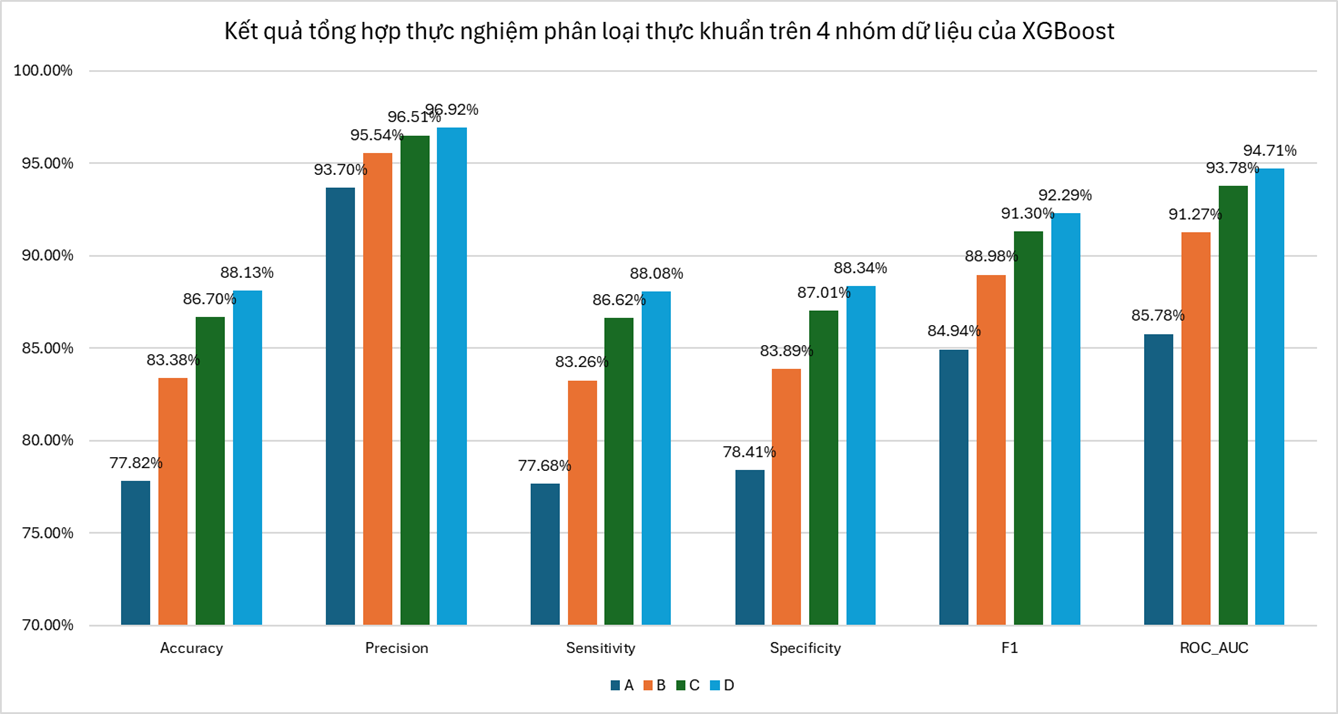
\includegraphics[width=1\linewidth]{figures/result_xgboost.png}
    \caption{Kết quả hiệu suất phân loại của mô hình XGBoost trên tập dữ liệu xây dựng.}
    \label{fig:result_2}
\end{figure}

\subsection{So sánh hiệu suất phân loại giữa DeePhage và XGBoost}

